\documentclass[../../thesis.tex]{subfiles}

\begin{document}

\section{MaskGIT}

The Masked Generative Image Transformer (MaskGIT)\cite{chang2022maskgit} is a generative transformer model for image synthesis developed by Google Research. The novelty of the model lies in the token generation. Unlike popular autoregressive generative transformers, who treat images as a sequence of tokens, MaskGIT introduces an image synthesis paradigm using a bi-directional transformer. This means that during training MaskGIT learns to predict tokens in all directions, an intuitively more natural way to consider images. At inference time MaskGIT starts out with a blank canvas and predicts the entire image, and iteratively keeps and conditions on the most confident pixels.\newline

MaskGIT assumes a tokenization procedure for stage 1. In the original paper \cite{chang2022maskgit} VQGAN \cite{VQGAN} was used and the actual contribution of the work revolved around improving stage 2, hence we present that part only. 

\subsection{Masked Visual Token Modeling (Prior learning)}

For prior learning the codebook learned in the tokenization procedure is provided with a masking vector, which is the embedding of the special masking token, which we denote by $\M$. The input embedding in the bidirectional transformer is initialized with this expanded codebook. For some image $X$ in the dataset $\mathcal{D}$, let $z = \{z_{k_i}\}_{i=1}^N$ denote the sequence of codewords obtained by passing $X$ through the VQ-Encoder. Such a sequence can equivalently be described as a sequence of indices $s = \{k_i\}_{i=1}^N$. The prior learning amounts to masking such a sequence and training the bidirectional transformer to predict the masked indices.
\newline

Let $s = \{k_i\}_{i=1}^N$ be the sequence of indices described above and denote the corresponding binary mask by $M = \{m_i\}_{i=1}^N$. During training a subset of $s$ is replaced by the masking token $\M$ according to the binary mask $M$. This is done by 

\begin{equation}
    s_\text{Mask} = s\odot (1_N-M) +  M\cdot\M,
\end{equation}

where $\odot$ is the Hadamard product, i.e point wise multiplication, and $1_N$ is a vector with the same shape as $M$ and $s$.\newline

The sampling procedure, or choice number of tokens to mask, is parameterized by a mask scheduling function $\gamma$. The sampling can be summarized as follows

\begin{itemize}
    \item Sample $r \sim U(0,1]$.
    \item Sample $\lceil \gamma(r)\cdot N \rceil$ indices $I$ uniformly from $\{0,\dots,N-1\}$ without replacement. 
    \item Create $M$ by setting $m_i = 1$ if $i\in I$, and $m_i = 0$ otherwise.
\end{itemize}

The training objective is to minimize the negative log likelihood of the masked tokes, conditional on the unmasked. 

\begin{equation}
    \loss_\text{Mask} = -\E_{s\in \mathcal{D}}\left[\sum_{i \in I} p(s_i|s_\text{Mask} ) \right]
\end{equation}

The bidirectional transformer is used to predict the probabilities $p(s_i|s_\text{Mask})$ of each masked token, and $\loss_\text{Mask}$ is computed as the cross entropy between the ground truth one-hot token and the predicted token.

\begin{figure}[h]
    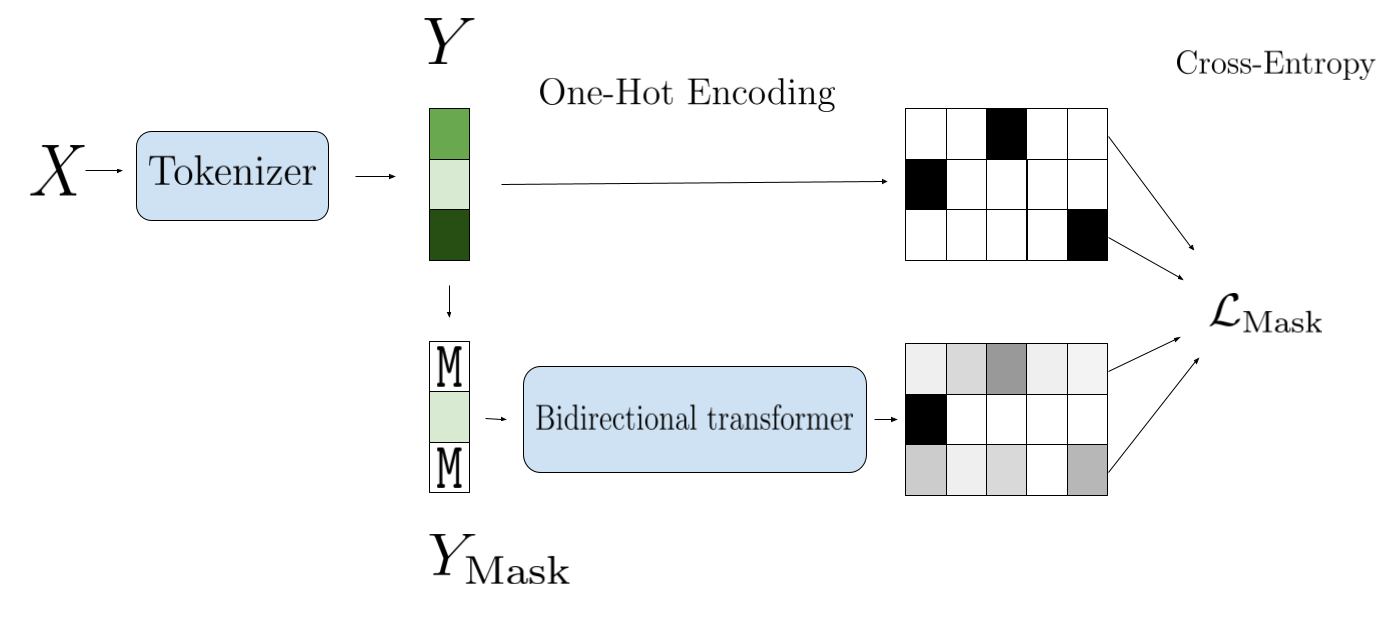
\includegraphics[scale=0.25]{MaskGIT.png}
    \centering 
    \label{fig:MaskGIT}
    \caption{MaskGIT forward computation.}
\end{figure}

\subsection{Iterative decoding (Image generation)}

The bi-directional transformer could in principle predict all $\M$ tokens and generate a sample in a single pass by simply sampling from the predicted probabilites $p(\widehat{s}_i|s_\text{Mask})$ from a forward pass of an all masked sequence. However, there are challenges with this approach. In their original article \cite{chang2022maskgit} proposes a novel non-autoregressive decoding method to synthesize samples in a constant number of steps.\newline

The decoding process goes from $t = 0$ to $T$. To generate a sample at inference time one starts out with an all masked sequence which we denote by $s_\text{Mask}^{(0)}$. At iteration $t$ the model predicts the probabilities for all the mask tokens, $p(\widehat{s}_i|s_\text{Mask}^{(t)})$, in parallel. At each masked index $i$ a token $s_i^{(t)}$ is sampled according to the predicted distribution, and the corresponding probability $c_i^{(t)}$ is used as a measure of the confidence in the sample. For the unmasked tokens a confidence of $1$ is assigned to the true position. The number of $s_i^{(t)}$ with highest confidence kept for the next iteration is determined by the mask scheduling function. We mask $n = \lceil \gamma(t/T)\cdot N \rceil$ of the lower confidence tokens by calculating $M^{(t+1)}$ by 

\begin{equation}
    m_i^{(t+1)} = 
    \begin{cases}
        1, \text{ if } c_i < \text{Sort}([c_1^{(t)},\dots,c_N^{(t)}])[n]\\
        0, \text{ otherwise} 
    \end{cases}
\end{equation}

\begin{figure}[h]
    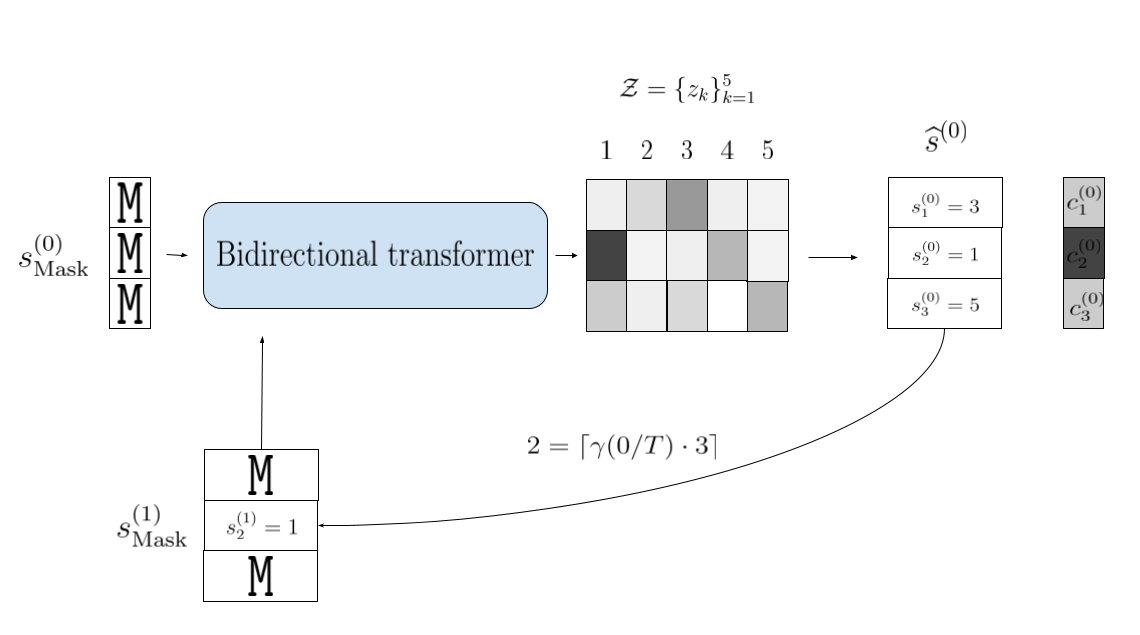
\includegraphics[scale=0.35 ]{Iterative Decoding.png}
    \centering 
    \label{fig:IterativeDecoding}
    \caption{Illustration of first pass of the iterative decoding algorithm.}
\end{figure}

The algorithm synthesizes a full image in $T$ steps. For image generation, cosine scheduling function proved best across all experiments in the original paper.


\section{TimeVQVAE}

TimeVQVAE is a time series generation model based on VQVAE and MaskGIT. It is the first to our and the authors knowledge that utilizes vector quantization (VQ) to address the TSG problem. It leverages a two stage approach similar to VQVAE and uses a bidirectional transformer akin to MaskGIT for prior learning. Additionally, they propose VQ modeling in time-frequency domain, separating data into high and low frequency components to better retain temporal consistencies and generate higher quality samples.\newline

TimeVQVAE provides class-guided conditional sampling. 

\subsection{Tokenization}

\begin{figure}[h]
    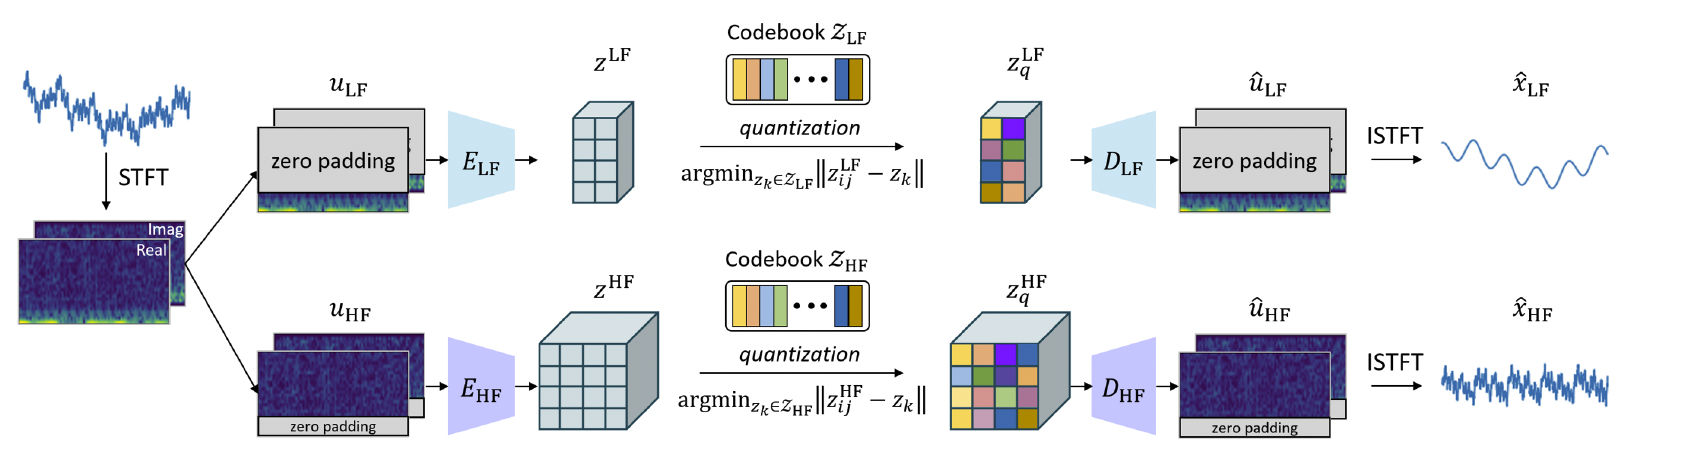
\includegraphics[scale=0.23]{TimeVQVAE1.png}
    \centering 
    \label{fig:TimeVQVAE1}
    \caption{Stage 1: Tokenization. Figure taken with permission from \cite{TimeVQVAE}}
\end{figure}

\subsection{Prior learning}

TimeVQVAE uses a modified version of MaskGIT in order to learn the prior. As the original MaskGIT has no means of jointly sample from the two modalities introduced by the high-low frequency split. \newline

For some  $X$ in the dataset $\mathcal{D}$, let $Y = \{y_i\}_{i=1}^N$ denote the latent tokens obtained by passing $X$ through the VQ-Encoder and denote the corresponding binary mask by $M = \{m_i\}_{i=1}^N$.\newline

A discrete latent representation $z_q \in \R^{d\times h\times w}$ can equivalently be represented as a sequence of codebook indices by 
\begin{equation}
    s_{ij} = k, \text{ whenever } (z_q)_{ij} = z_k
\end{equation}

% \begin{figure}[h]
%     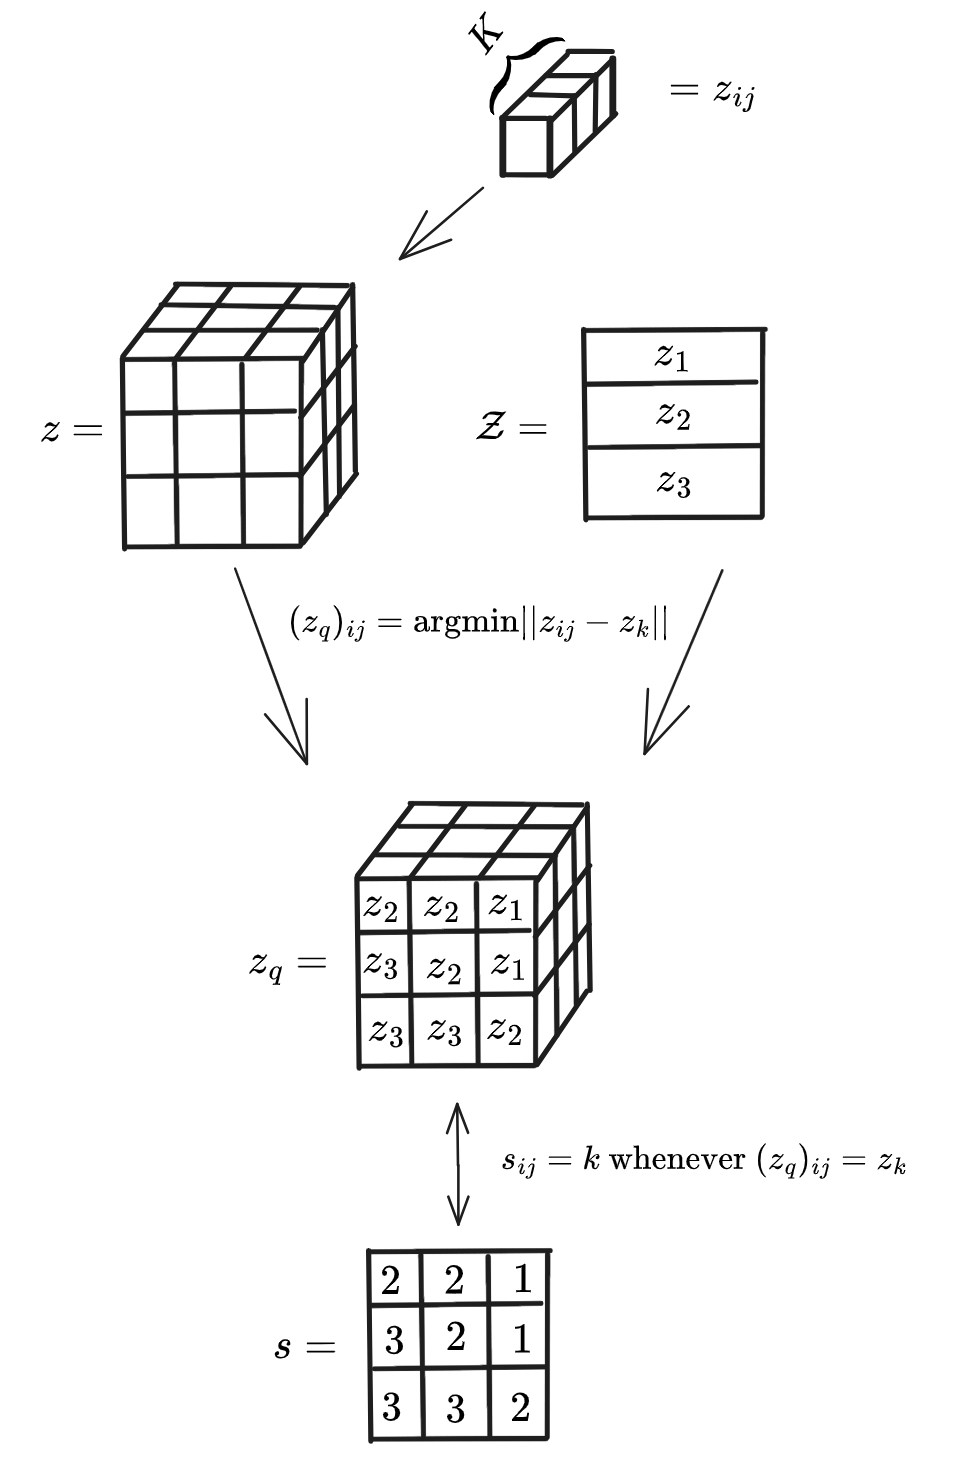
\includegraphics[scale=0.2]{quantization}
%     \centering    
% \end{figure}



\subsubsection{Class Conditional Sampling}

The prior is learned such that the model can generate synthetic samples both conditionally and unconditionally. By appending a class token, similarly to \cite{dosovitskiy2021image}, 

\section{SSL}

Our model leverages SSL algorithms in order to learn more expressive latent representations. Here we present the relevant algorithms for our work, Barlow Twins and VIbCReg.
\newline
One fundamental difference between Barlow Twins and VIbCReg is that the branches are regularized differently. In Barlow Twins the regularization is applied to the cross correlation matrix of the projected output of the two branches, which in general favours scenarios where the two branches produces similar summary statistics. In VIbCReg the covariance term is applied on each branch separately, which works better in scenarios where the branches are different \cite{bardes2022vicreg}.

\subsection{Barlow Twins}
Barlow Twins is a non-contrastive SSL method based on applying the \textit{redundancy-reduction principle} (or efficient coding hypothesis) \cite{Barlow_origin} from the neuroscientist H. Barlow to a pair of identical networks.\newline  

In essence the model wants to encourage representations of similar samples to be similar, while simultaneously reducing the amount of redundancy between the components of the vectors. This is enforced by producing two augmented views of each sample and projecting the their representations onto a vast feature space, in such a way that their cross-correlation is close to the identity. \newline

\begin{figure}[h]
    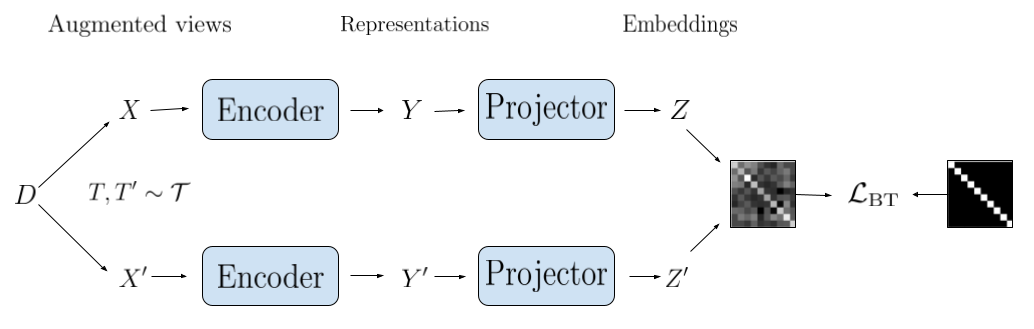
\includegraphics[scale=0.35]{BarlowTwins.png}
    \centering    
    \caption{Overview of the Barlow Twins architecture. Figure inspired by \cite{zbontar2021barlow}}
\end{figure}

The Barlow Twins algorithm starts out by creating two different augmented views for each datapoint in a batch $D$. The augmentations are selected by sampling from a collection of augmentations $\mathcal{T}$. We denote the batches of augmented views $T(D) = X$ and $T'(D) =X'$, for augmentations $T,T'\sim \mathcal{T}$.  The batches are then passed through an encoder (give representations $Y$ and $Y'$) and a \textit{projector} to produce batches of embeddings $Z$ and $Z'$. The embeddings are assumed to be mean centered across the batch dimension. \newline

The loss function is calculated using the cross correlation matrix $\C$ between $Z$ and $Z'$, and measuring its deviance from the identity. In particular the Barlow Twins loss is defined as

\begin{equation}
    \label{eq:BTLoss}
    \loss_{\text{BT}} = 
    \overbrace{\sum_i (1 - \C_{ii})^2}^{\text{Invariance}}
    +\lambda  \overbrace{\sum_i\sum_{j\neq i} \C_{ij}^2}^{\text{Redundancy reduction}},
\end{equation}
where
\begin{equation}
    \C_{ij} = \frac{\sum_b z_{b,i}z_{b,j}'}{\sqrt{\sum_b (z_{b,i})^2}\sqrt{\sum_b (z_{b,j}')^2}}.
\end{equation}

The \textit{invariance term} assists in making the embedding invariant to the distortions introduced by the augmentations, hence pushes the representations closer together. The \textit{redundancy reduction term} decorrelates the different vector components, which reduces the information redundancy. \newline



\subsection{VIbCReg}

VIbCReg \cite{lee2024vibcreg} is a non-contrastive SSL model with siamese architecture based on VICReg \cite{bardes2022vicreg}. It can be seen as VICReg with better covariance regularization and IterNorm \cite{huang2019iterative}. Overall the architecture is similar to Barlow Twins, but a key difference is that variance/covariance regularization is done in each branch individually.\newline

As before a batch $D$ is augmented to create two views and passed through an encoder and projector. The embedding $Z$ and $Z'$ are \textit{whitened} \todo{define or elaborate on this} using IterNorm \cite{huang2019iterative}.\newline

\begin{figure}[h]
    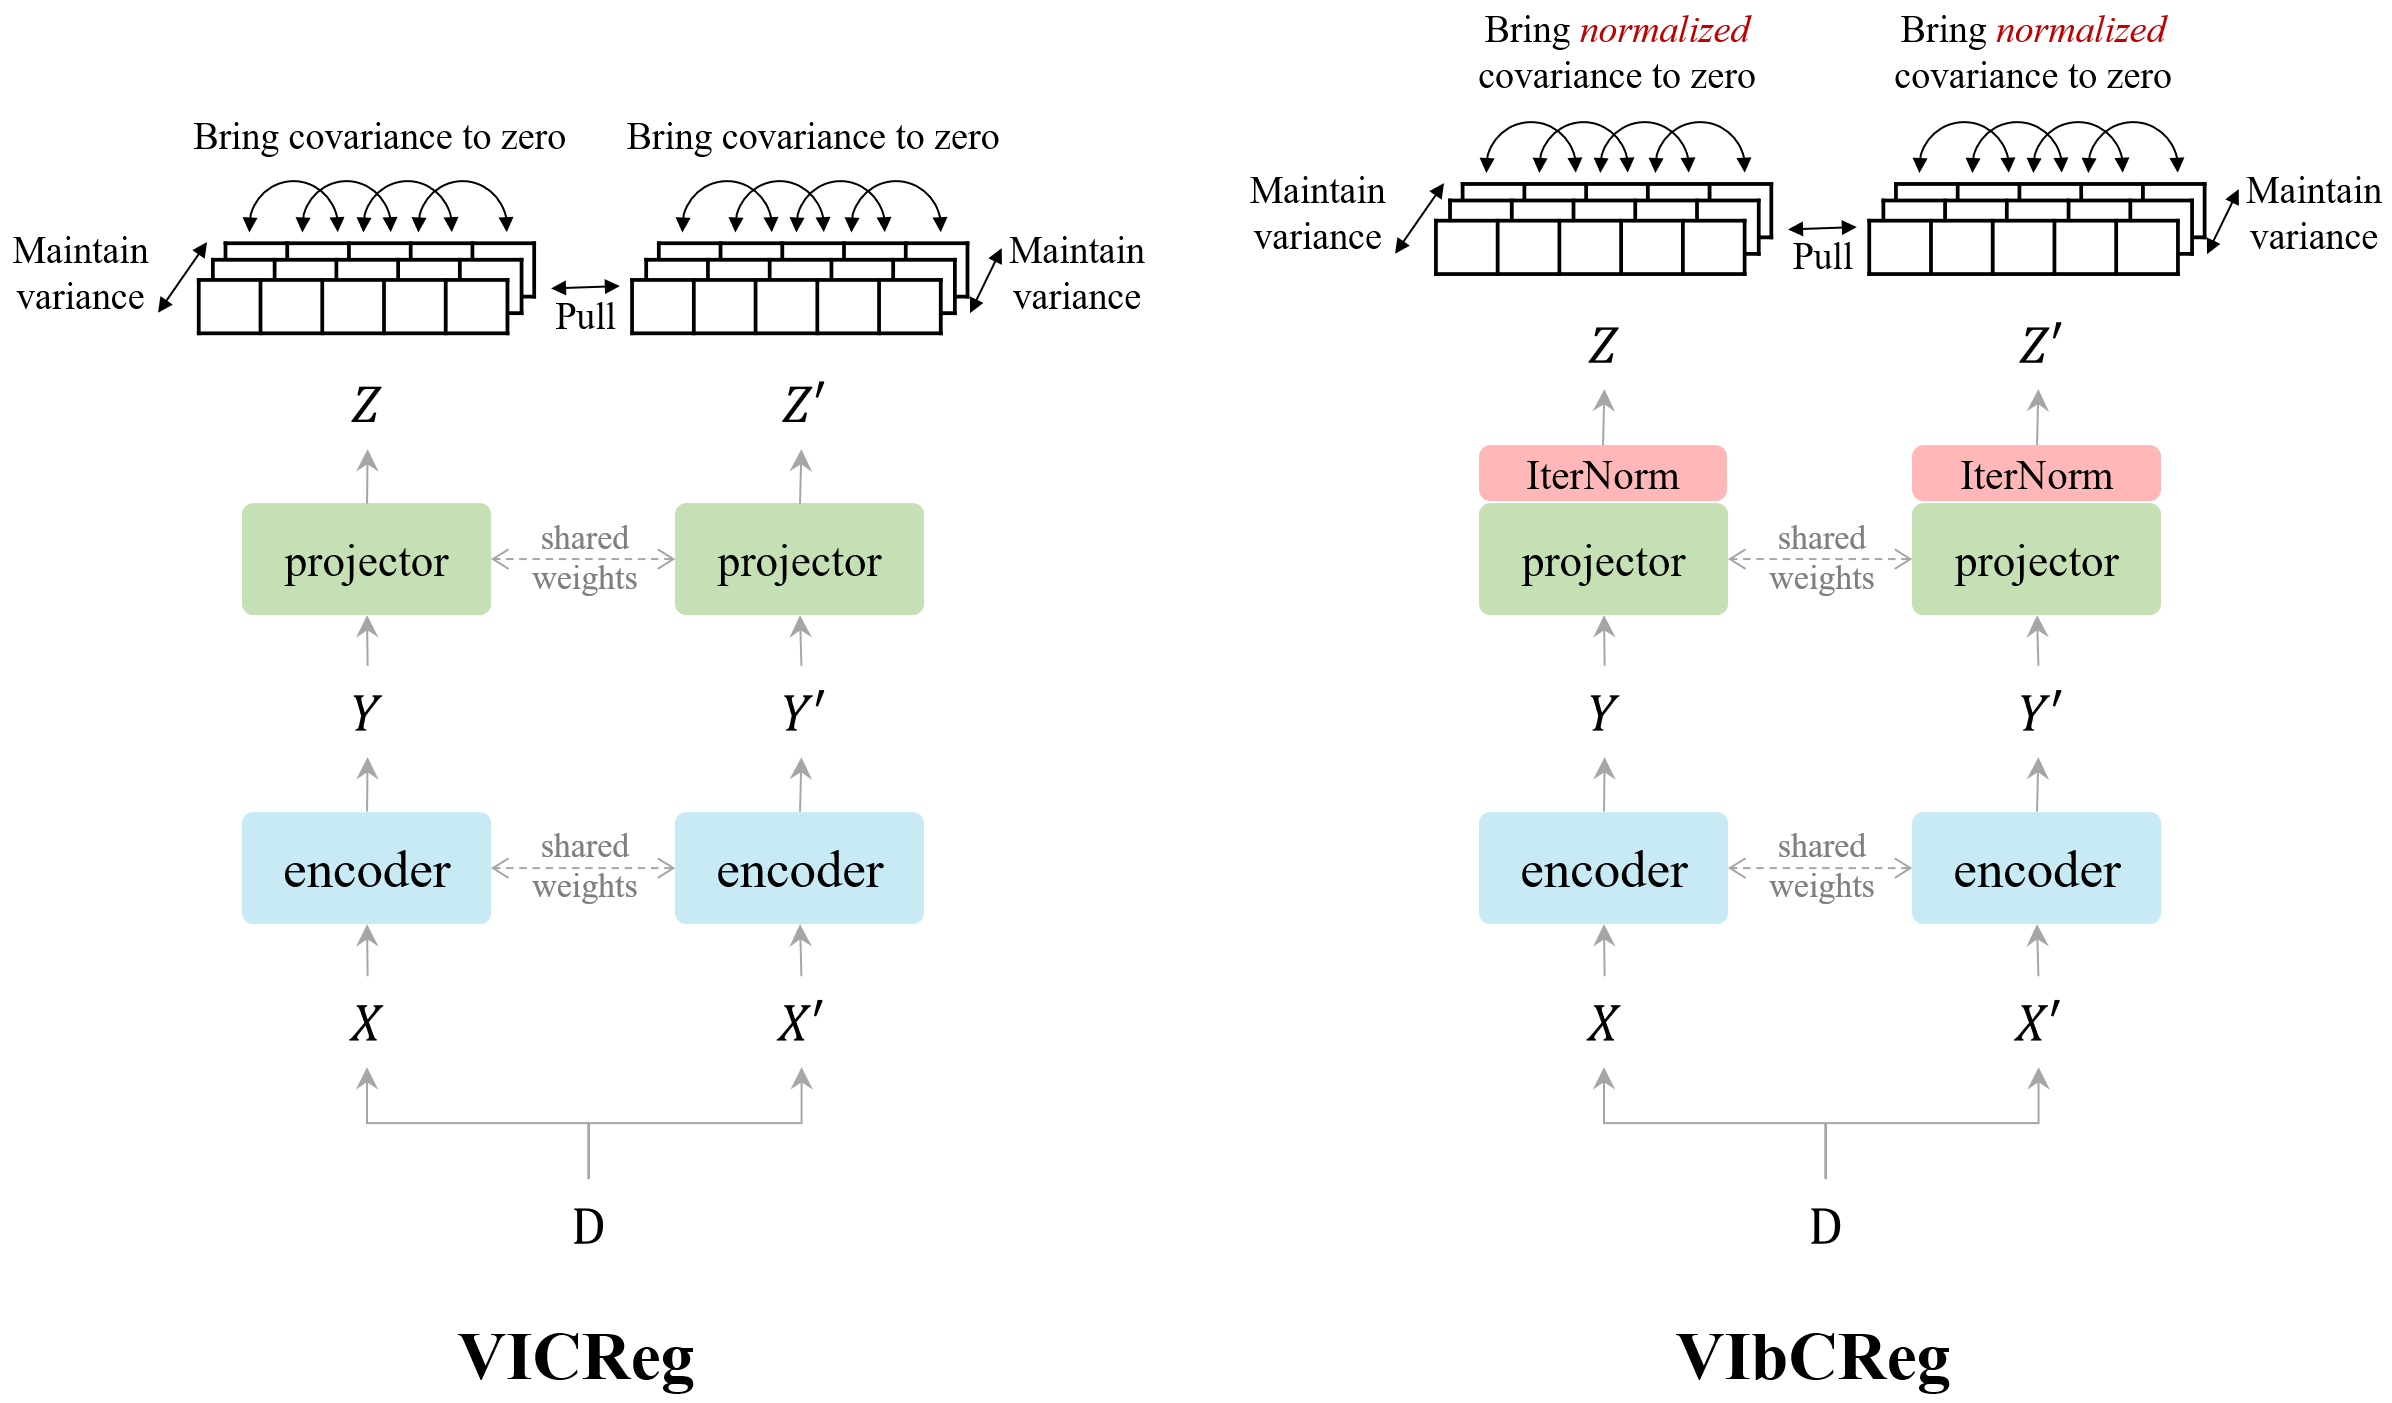
\includegraphics[scale=0.15]{VICReg_VIbCReg.png}
    \centering    
    \caption{Overview of VIbCReg, and comparison with VICReg. Taken with permission from \cite{lee2024computer}}
\end{figure}

The loss consists of a similarity loss between the branches, and feature decoration (FD) loss together with a feature component expressiveness (FcE) term at each branch. Input data is processed in batches. Let $Z \in \mathbb{R}^{B\times F}$ where $B$ and $F$ denotes the batch and feature sizes respectively. We denote a row in $Z$ by $Z_b$ and column by $Z_f$, and similarly for $Z'$. \newline

The similarity loss is defined as the MSE of the two embeddings

\begin{equation}
    s(Z,Z') = \frac{1}{B} \sum_{b=1}^B || Z_b-Z_b'||_2^2,
\end{equation}
which encourages them to be similar. The FcE term acts on each branch separately and encourages the variation across a batch to stay at a specified level $\gamma$. It is defined as 
\begin{equation}
    v(Z) =  \frac{1}{F} \sum_{f=1}^F \max(0,\gamma - \sqrt{\text{Var}(Z_f)+\epsilon}),
\end{equation}
where $\text{Var}()$ is a variance estimator, $\gamma$ is a target value for the standard deviation, which both in VIbCReg and VICReg is set to $1$. $\epsilon$ is a small scalar preventing numerical instabilities. 
\newline 
For the FD loss we first mean shift and normalize along the batch dimension
\begin{equation}
    \widehat{Z}_b = \frac{Z_b-\bar{Z}}{||Z_b-\bar{Z}||_2} \text{ where }  \bar{Z} = \frac{1}{B}\sum_{b=1}^B  Z_b,
\end{equation}
\begin{equation}
    \widehat{Z} = [\widehat{Z}_1,...,\widehat{Z}_B]^T,
\end{equation}
compute the normalized covariance matrix
\begin{equation}
    C(Z) = \frac{1}{B-1}\widehat{Z}^T \widehat{Z},
\end{equation}
and take the mean square across all off-diagonal elements to obtain the FD loss
\begin{equation}
    c(Z) = \frac{1}{F^2}\sum_{i\neq j} C(Z)_{ij}^2.
\end{equation}
The total loss is then given by
\begin{equation}
    \label{eq:VIbCRegLoss}
    \loss_\text{VIbCReg} = \lambda s(Z,Z') + \mu [v(Z) + v(Z')] + \nu[c(Z)+c(Z')]
\end{equation}
where $\lambda, \mu$ and $\nu$ are hyperparameters determining the importance of each term. The normalization of the covariance matrix keeps the range of the FD loss small, independent of data, and eases hyperparameter tuning across datasets.
% \begin{equation}
%     C(Z) = \frac{1}{B-1} \left(\frac{Z-\bar{Z}}{||Z-\bar{Z}||_2}\right)^T\left(\frac{Z-\bar{Z}}{||Z-\bar{Z}||_2}\right) \text{ where }  \bar{Z} = \frac{1}{B}\sum_{b=1}^B  Z_b
% \end{equation}




\end{document}